
\documentclass[9pt]{IEEEtran}

% basic
\usepackage[english]{babel}
\usepackage{graphicx,epstopdf,fancyhdr,amsmath,amsthm,amssymb,url,array,textcomp,svg,listings,hyperref,xcolor,colortbl,float,gensymb,longtable,supertabular,multicol,placeins}
\usepackage{diagbox}
 % `sumniki' in names
\usepackage[utf8x]{inputenc}
\usepackage{multirow}
\usepackage{makecell}

 % search and copy for `sumniki'
\usepackage[T1]{fontenc}
\usepackage{lmodern}
\input{glyphtounicode}
\pdfgentounicode=1

% tidy figures
\graphicspath{{./figures/}}
\DeclareGraphicsExtensions{.pdf,.png,.jpg,.eps}

% correct bad hyphenation here
\hyphenation{op-tical net-works semi-conduc-tor trig-gs}

% ============================================================================================

\title{\vspace{0ex} %
% TITLE IN HERE:
Implemetation and evaluation of QRS complex detection with the Chen algorithm
\\ \large{Assignment \#1}\\ \normalsize{Biometrical signal and image processing 2020/21, Faculty of Computer and Information Science, University of Ljubljana}}
\author{ %
% AUTHOR IN HERE:
Žiga~Kleine
\vspace{-4.0ex}
}

% ============================================================================================

\begin{document}

\maketitle

\begin{abstract}

In this report, I will present my QRS complex detector, based on the article from HC Chen and SW Chen \cite{chen2003moving}. For the implementation, I used the MATLAB programming framework, which includes many functions useful for digital signal processing. I evaluated the algorithm on the Long-Term ST Database, using the wfdb software package functions bxb and sumstats \cite{jager2003long, goldberger2000physiobank}. I followed the algorithm described in the paper, that means that the signal first goes trough a linear high-pass filter, then trough a non-linear low-pass filter, and then lastly, the QRS complexes are detected through adaptive thresholding.

\end{abstract}

\section{Introduction}

QRS complex detection in heartbeats is a problem that has been tackled by scientists since the late seventies. Since the eighties it has been running on home computer chips in real time \cite{pan1985real}. It is usually implemented with a series of filters.
The Chen agorithm is no different \cite{chen2003moving}. It consists of three parts, a linear high-pass filter, described by the difference equation \ref{eq:1},  and a non-linear low-pass filter, implemented with a cascade of a simple
point-by-point squaring operation and a moving window summation system, then lastly, the detection part of the algorithm, which uses adaptive thresholding to detect fiducial points in the QRS complexes of the heartbeat ECG.

\section{Methodology}

As mentioned, I implemented the algorithm in the MATLAB environment. I implemented the first part, the high-pass filter, by using the filter() function in MATLAB. I used the M value of 7. Then the signal goes through the low-pass filter, which was implemented by first squaring all values in the signal and then performing a moving window summation, implemented with the MATLAB movsum() function. I used the moving summation window of size 32. Then the QRS complex detection was implemented with the help of the adaptive thresholding function \ref{eq:2}. As the article suggests, i used the value of  $ \alpha  = 0.05 $ and  $ \gamma = 0.15 $. The first PEAK value was found by calculating the mean of all peaks found by the findpeaks() function on the first 5000 samples of the input ECG signal. Then, the algorithm found the peak indexes by searching for the index of the maximum value of the region when the signal exceeds the threshold value. When a new peak was found, the threshold value was updated accordingly. 

The result of the detection was then evaluated by comparison to the annotations in the whole LTST database. This was done with the help of bxb and sumstats programs in the wfdb software package. We will discuss the value of averaged metrics of Sensitivity \ref{eq:3} and Positive Predictivity  \ref{eq:4} on all of the recordings in the LTST database.

\begin{equation} \label{eq:3}
Se =  \dfrac{TP}{TP + FN} 
 \end{equation}

\begin{equation} \label{eq:4}
+P =  \dfrac{TP}{TP +FP} 
 \end{equation}

I then tried to improve the detection. The first obvious improvement that came to mind was to use all of the signals included in the recording and not just the first one, as I did at first. I simply calculated the average of the signals included by first summing the signals in the recording and then divided them by the number of the signals present. It improved the QRS complex detection.

The second improvement I firstly achieved by a mistake in my code, where I skipped over a few samples just after the end of the detected QRS complex. I found out that if I skipped a few samples after the end of the detected QRS complex, the Positive Predictivity of the algorithm evaluated on the database increased significantly, while the Sensitivity decreased by a marginal amount. 

\begin{equation} \label{eq:1}
 y[n] =  x[ n - \dfrac{M +1}{2}]  - \dfrac{1}{M}*\sum_{m=0}^{M-1}x[m-n] 
 \end{equation}

\begin{equation} \label{eq:2}
Threshold = \alpha*\gamma* PEAK - (1 - \alpha)*Threshold  
\end{equation}

\begin{figure}[!htb]
\centering
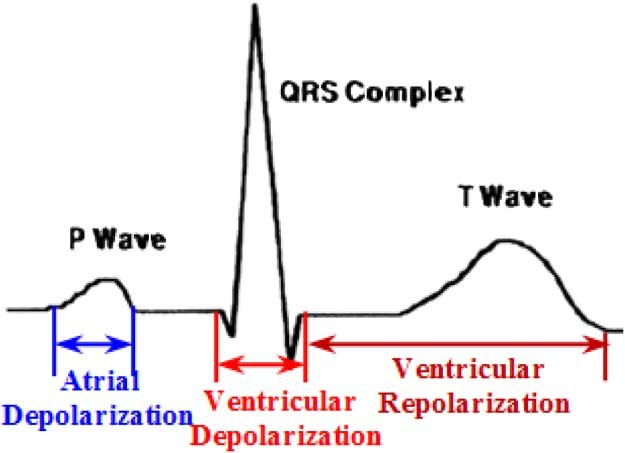
\includegraphics[width=1\columnwidth]{heartbeat.png}
\caption[c1]{ Parts of the heartbeat. }
\label{fig_sim1}
\end{figure}

\section{Results}

The worst results were achieved by just the basic algorithm that was ran on just the first signals in their respective recordings. The better result, which also has the best positive predictivity of all of them was achieved by running the Chen algorithm on the averaged signal of all of the signals in the recording. Then by sacrificing a small margin of the Sensitivity, the Positive Predictivity metric increased by quite a lot by skipping a few samples after the end of the succesfully detected QRS complex \ref{table2}. My theory is that the algorithm sometimes wrongly detects the T-wave or the ventricular repolarization as the actual QRS complex, and skipping a few samples improves that \ref{fig_sim1}.

\begin{table}[!htb]
\scriptsize
\renewcommand{\arraystretch}{1.3}
\centering
\begin{tabular}{|c||c|c|}\hline
\bf{Algorithm} & \bf{Sensitivity} & \bf{Positive Predictivity} \\ \hline \hline 
 \makecell{Chen algorithm \\ on one signal }  & 96.91 & 93.13 \\ \hline
 \makecell{Chen algorithm \\ on averaged signal } & 98.27 & 96.35 \\ \hline
 \makecell{Averaged signal \\ with 20 skipped samples}  & 98.24 & 97.87 \\ \hline
 \makecell{Averaged signal \\ with 25 skipped samples}   & 98.23 & 97.98 \\ \hline
 \makecell{Averaged signal \\ with 30 skipped samples}  & 98.19  & 98.11 \\ \hline
 \makecell{Averaged signal \\ with 35 skipped samples}  & 98.19  & 98.11 \\ \hline
\end{tabular}
\caption{Performance of the Chen algorithm and my improvement attempts. }
\label{table2}
\end{table}

\section{Discussion}

The implemented Chen QRS complex detector works well with over 98 percent Positive Predictivity and Sensitivity on the LTST database. The algorithm can be improved by introducing a more complex filtering and detection pipeline. My improvement with sample skipping could probably be improved by keeping track of the heart rate and then skipping an appropriate amount of samples.

\bibliographystyle{IEEEtran}
\bibliography{bibliography}

\end{document}